% !TeX encoding = UTF-8
%% (requires IEEEtran.cls version 1.7 or later) with an IEEE conference paper.
\documentclass[journal]{IEEEtran}

\renewcommand\IEEEkeywordsname{Keywords}

\pagenumbering{gobble}

\usepackage[utf8]{inputenc}

% *** GRAPHICS RELATED PACKAGES ***
%\usepackage[pdftex]{graphicx}
\usepackage{graphicx}
%\usepackage[dvips]{graphicx}
% to place figures on a fixed position
\usepackage{float}

% *** PDF, URL AND HYPERLINK PACKAGES ***
\usepackage{url}

% correct bad hyphenation here
%\hyphenation{}

\usepackage{xcolor}



% \renewcommand\note[1]{} % uncomment this line to hide notes

%%%%%%%%%%%%%%%%%%%%%%%%%%%%%%%%%%%%%%%%%%%%%%%%%%%
%%%%%%%%%%%%%%%%%%%%%%%%%%%%%%%%%%%%%%%%%%%%%%%%%%%
%%%%%%%%%%%%%%%%%%%%%%%%%%%%%%%%%%%%%%%%%%%%%%%%%%%
%


% LaTeX quick ref
%
% \cite{refname} to place citation
%
% \label{label_name} to place a label, which can be reference by \ref{label_name}
%
% new paragraph -> empty line between text
%
% \noindent to not indent paragraphs first line
%
% create list with : \begin{itemize} \end{itemize}
% \begin{itemize
% \renewcommand to renew numbering \labelitemi{--} to select bullet type
% \item item elem 1
% \item item elem2
% \end{itemize}
%
% et alia (et al.) should be emphasized (i.e in italic) with \emph{et al.}
%
% to add figure, htb is placement selector , !overrid internal paramters
%\begin{figure}[!htb]
%    \centering
%    \includegraphics[width=0.5\textwidth]{FIG.png}
%    \caption{Caption}
%    \label{fig:label}
%\end{figure}
%
% ~ concatenates dynamic text with literals
%
% long dash is --
%
% `is single quoted' , ``is double qouted"
%
% to autoformat with latexindent: latexindent -w  -m -l defaultSettings.yaml ProtoImplFPGA.tex


\begin{document}
% conference papers do not typically use \thanks and this command
% is locked out in conference mode. If really needed, such as for
% the acknowledgment of grants, issue a \IEEEoverridecommandlockouts
% after \documentclass
% paper title
% can use linebreaks \\ within to get better formatting as desired
\title{A Flexible Architecture for Protocol Implementations within FPGAs}
%\titleheader{25th Telecommunications forum TELFOR 2017 \hfill Serbia, Belgrade, November 21-22, 2017.}

% author names and affiliations
% use a multiple column layout for up to three different
% affiliations
\author{Ferenc Nándor Janky\thanks{Ferenc Nándor Janky	is with Dept. of Telecommunications and MediaInformatics,
        Faculty of Electrical Engineering and Informatics, Budapest University of Technology and Economics, Magyar tudósok
        körútja 2., 1117 Budapest, Hungary (phone: +36704213213; e-mail: fecjanky@gmail.com)}%
}%

\markboth{25th Telecommunications forum TELFOR 2017 \hfill Serbia, Belgrade, November 21-22,
    2017.}%
{}

\IEEEpubid{\makebox[\columnwidth]{978-1-5386-3073-0/17/\$31.00~\copyright~2017 IEEE\hfill}
    \hspace{\columnsep}\makebox[\columnwidth]{ }}

% make the title area
\maketitle

\begin{abstract}
    \boldmath
    The handling of networking protocol messages that has low memory footprint could be implemented
    effectively by using FPGAs.

    The purpose of this work was to design a generalized approach for implementing protocols using FPGA hardware.
    %In order to validate the approach, this paper also presents an application layer protocol that was implemented
    %through
    %using the generalized architecture as a framework.

    %The ISO OSI Basic Reference Model~\cite{ISO:OSI} for communication is a remarkable guideline as a design basis for
    %setting the
    %boundaries of such a generalized architecture. As a result of this work, a framework has been designed and also
    %described in VHDL. It  follows the basic principles of the OSI reference, presenting a general tool-kit for
    %handling
    %PDUs (Protocol Data Units) and IDUs (Interface Data Units). Beside these features it also provides solutions
    %for other
    %frequently reappearing tasks in the aid of convenient and smooth implementation of various protocols.

    %%%%%%%% To verify the design a partial implementation of SNMP and various other lower layer protocols have been implemented
    %%%%%%%% which was interconnected with with other link, network and transport layer hardware and software products from 3rd 
    %%%%%%%% party vendors. The conformance testing of the SNMP implementation had been carried out with a couple of network 
    %%%%%%%% management software.

    The model has been verified through simulations as well as through physical, live tests. The simulations were
    performed on the VHDL description itself. The live tests were carried out on the fully implemented application of
    ARP
    and Ethernet, which was interconnected with network and transport layer hardware and software products from 3rd
    party
    vendors.
\end{abstract}

\begin{IEEEkeywords}
    FPGA, Networking, Protocol stack, VHDL
\end{IEEEkeywords}

% no keywords
\section{Introduction}\label{sec:Motivation}

The family of connectionless low memory footprint networking protocols can be handled with relative ease by having pure
hardware-based implementations using FPGAs.

One of the greatest motivation of having hardware based protocol implementations is to provide deterministic timing
characteristics. This is essential for several networking protocols such as Time Triggered Ethernet~\cite{SAE_AS6802},
whereas time synchronization protocols like PTP (Precision Time Protocol) \cite{PTP_standard}could also benefit from
them.

There could be various focal points for FPGA-based networking equipment design; these include high networking speed
\cite{C-GEP_HPSR} low latency \cite{related:TrustNode}, ease of programmability \cite{C-Board_NEMA}, etc.

There are many networking solutions available for NetFPGA \cite{NetFPGA}, which is a widely used platform
in research and education. Naturally, there are many protocol-implementations available for NetFPGA users, although
their implementations are heterogeneous, which forces the developer to take extra special care when stacking up
protocols.

All of these solutions essentially need protocol handling within the FPGA. Most FPGA manufacturers provide black box
modules of which several protocols can be synthesized. While these can be used well with well-established protocols,
their rigid nature makes them inappropriate for protocol development.
In real life there are often non-existing features
or new protocols have to be implemented, for which the factory-provided implementations allow little design space.
Often times there are only some generic parameters of a given protocol that can be tweaked as a part of instantiation.
For new protocols, the implementation process usually follows a practically ad-hoc method that may come with special
advantages of tailoring, but definitely needs longer design time.
This includes developing the given protocol logic, and rather than fitting that into a generic interface,
the designer has to fit that into the stack as the \emph{implementation} of the surrounding protocols require.

In order to speed up design time and provide a clear solution, a systematic approach is suggested in this paper,
that follows the layered OSI model~\cite{ISO:OSI} of communication.

The motivation for this work is to design and implement a framework in VHDL that enables rapid prototyping of
networking protocols. The aim is not to provide similar black box modules, but to supply elementary components in a way
that the implementer could only focus in designing and implementing the protocol specific parts. The ISO OSI model
provides a standard way of talking about protocols. As a result, lining up the design of the framework with the OSI
model is a straightforward decision. Besides, it provides a well-established nomenclature, and it also lays down the
fundamentals of the modular architecture of the framework.

\IEEEpubidadjcol

\section{Internal Design}\label{sec:Internal Design}

The internal design of the framework aligns with the OSI model, as mentioned before. Individual layers of protocols
communicate through SAPs (Service Access Points), using service primitives.
These mostly have protocol dependent parameters, but their structure is fixed and consists of ICI (Interface Control
Information) and SDU (Service Data Unit). Given these, it is beneficial to have a generic component that can be reused
in each and every protocol for handling ICIs,SDUs and PDUs. The designer's task is to implement:
%(i)the protocol operation as specified,
%(ii)the interface towards upper layer protocols, and
%(iii)the interface towards lower layer protocols.
\begin{itemize}
    \renewcommand \labelitemi{--}
    \item the protocol operation as specified,
    \item the interface towards upper layer protocols, and
    \item the interface towards lower layer protocols.
\end{itemize}

Such a straightforward approach help minimizing implementation errors, and reducing verification effort.

Based on the description above the framework essentially becomes a generic module or building block, that has some
clear properties, that
%(i)has to support interconnection via layering;
%(ii)handles reception and transmission of PDUs with queuing;
%(iii)provides a high level interface for separating and combining PCI (Protocol Control Information) and SDU,
%(iv)forwarding, pausing or dropping SDUs;
%(v)provides a unified way to handle ICI, SDU, and PDU events (e.g error signalling);
%(vi)adds support of auxiliary information that travels along with messages -- this can be used for adding meta-data to message or in creating SAPs;
%(vii)provides components for common tasks recurring during implementing networking protocols and (de/serialization, arbitration etc.).
\begin{itemize}
    \renewcommand \labelitemi{--}
    \item has to support interconnection via layering;
    \item handles reception and transmission of PDUs with queuing;
    \item provides a high level interface for separating and combining PCI (Protocol Control Information) and SDU,
          forwarding, pausing or dropping SDUs;
    \item provides a unified way to handle ICI, SDU, and PDU events (e.g error signalling);
    \item adds support of auxiliary information that travels along with messages -- this can be used for adding
          meta-data to message or in creating SAPs;
    \item provides components for common tasks recurring during implementing networking protocols
          (de/serialization, arbitration etc.).
\end{itemize}

Fig.~\ref{fig:system_sketch} shows the high level design of the Protocol Layer module. The PUI and PIP part is
interconnected via a control and a data bus. The control signals provide a way for signalling various conditions: start
of PDU, end of PDU, etc. All of the module's buses are configurable via generics in terms of:
\begin{itemize}
    \renewcommand \labelitemi{--}
    \item bus width,
    \item handshake or unsolicited mode of Tx/Rx,
    \item number of messages to queue,
    \item instantiation of auxiliary queue for Tx/Rx.
\end{itemize}

\begin{figure}[!htb]
    \centering
    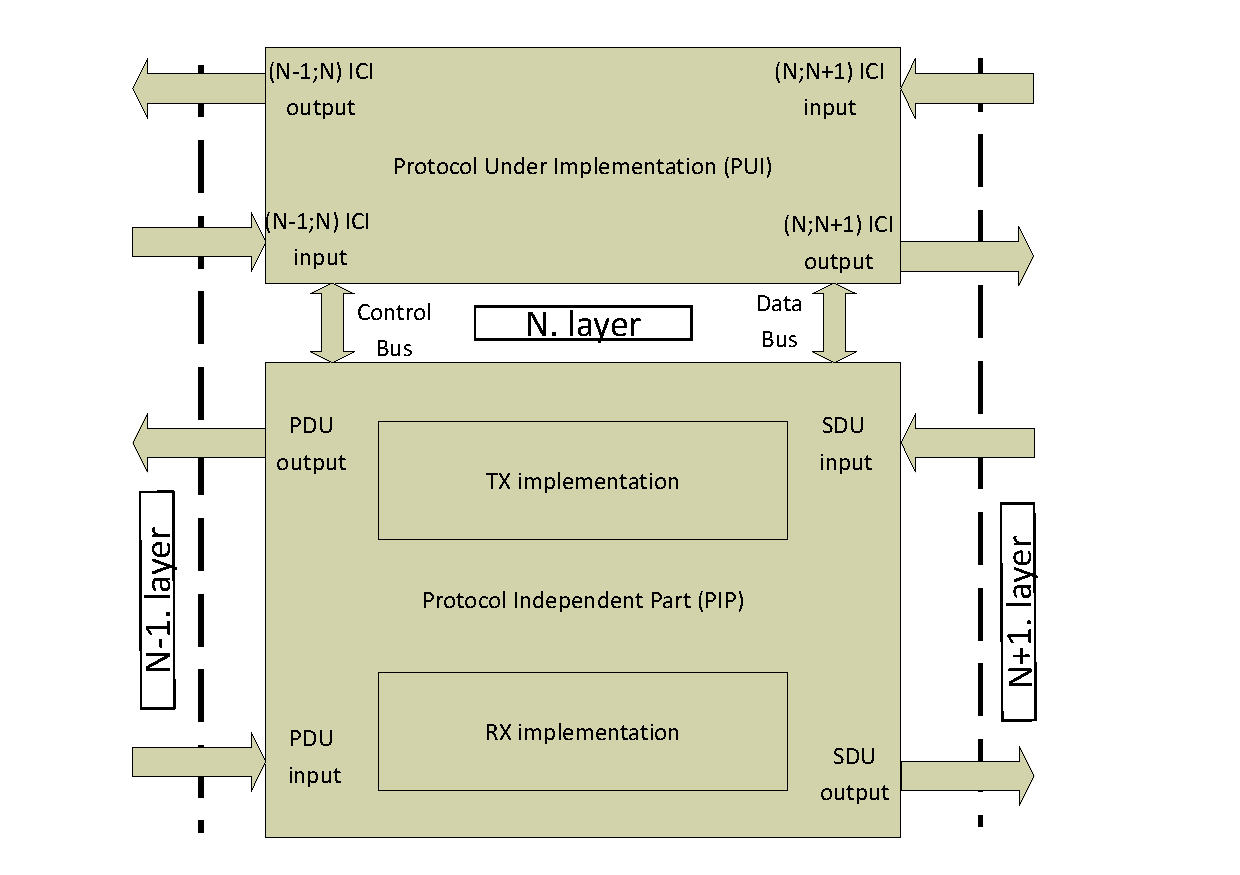
\includegraphics[width=0.4\textwidth]{figures_raw/system_sketch.pdf}
    \caption{Generic overview of the fundamental building block of the framework}
    \label{fig:system_sketch}
\end{figure}

\subsection{Interface and functional specification of the VHDL modules}\label{subsec:if_and_func_spec_VHDL}

\subsubsection{Handshaking mechanism and error signalling}
In synchronous systems there is a need for handshaking to indicate a request for certain operations to be carried out.
In this framework this is generalized into having two signals: \emph{Ind} and \emph{Ack}.
\emph{Ind} is used for indicating a request, whereas \emph{Ack} is for providing acknowledgement for
the requested operation. All synchronous operations must be carried out after receiving an \emph{Ack}.
Synchronous operation is not always preferable -- e.g. when there is only one upper layer protocol in a
given system. That is the reason why every interface is parametrizable with generics whether to use
handshaking or not.
Beside the bidirectional data and control buses, there are bidirectional error indicator signals present
for signalling error conditions for both parties of the communication.

\subsubsection{Data delimiter signals}

Data is traversing through the system in the form of consecutive bytes over various data buses (PDU, internal data,
aux. data etc.) accompanied by:
\begin{itemize}
    \renewcommand \labelitemi{--}
    \item Start Of PDU control signal (SOP),
    \item End of PDU control signal (EOP),
    \item Data Valid control signal (DV).
\end{itemize}
If a module is transferring data, it must indicate it by transitioning both SOP and DV signals from logical `Low' to
`High' level simultaneously -- and in parallel, the data bus is also adjusted to the first symbol of the data to be
sent.
If a module samples SOP and DV on a rising edge of the clock, then it can shift in and start processing the data from
the data bus when DV is `High' (among other things that can be used as a write enable signal).
The end of data is signalled by a pulse on the EOP line while DV is `High'. After this, all control signals have to be
settled on `Low' logical level.

\subsubsection{Combining handshaking, error handling and delimiters}

Fig.~\ref{fig:data_signals} illustrates data transfer combined with synchronization. The delimited data transfer must
take place after the \emph{Ind}-\emph{Ack} handshake.
%%%%%%%% i.e.when the sending component samples `High' on the \emph{Ack} wire --  while the receiver can withhold the 
%%%%%%%% acknowledgement indefinitely -- the sender must only reset the indication signal if an error is signalled. 
%%%%%%%% ezt nem értem, mire példa, miért kell ide... (?)%
The source module can cancel the transmission by transitioning the \emph{Ind} signal back to `Low' level. After the
handshake, the data transmission must take place. After a successful handshake the sender can only cancel the
transmission through a signalling error.

%%%%%%%%  WaveDrom waveform to generate figure http://wavedrom.com/editor.html
%%%%%%%% {signal: [
%%%%%%%%   {name: 'CLK', wave: 		'P........|.....'},
%%%%%%%%   {name: 'Ind', wave: 		'0.1..0...|.....'},
%%%%%%%%   {name: 'Ack', wave: 		'0..1.0...|.....'},
%%%%%%%%   {name: 'SOP', wave: 		'0...10...|.....'},
%%%%%%%%   {name: 'EOP', wave: 		'0........|..10.'},
%%%%%%%%   {name: 'DV', wave:  		'0...1....|...0.'},
%%%%%%%%   {name: 'DATA[x:0]', wave: 'x...3....|...x.', data: ['data']},
%%%%%%%% ]}
\begin{figure}[!htb]
    \centering
    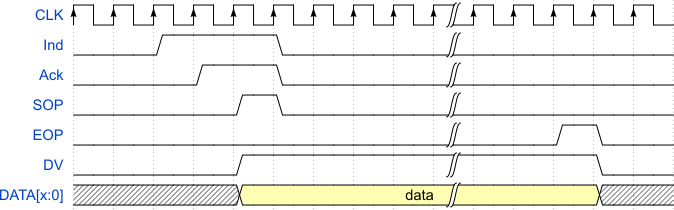
\includegraphics[width=0.45\textwidth]{figures_raw/data_signals.png}
    \caption{Waveform of a typical, error free data transmission between modules}
    \label{fig:data_signals}
\end{figure}

\subsection{Detailed design of Protocol layer module}

\subsubsection{Detailed design of \emph{`PDUQueue'}}\label{subsubsec:PDUQueue_details}

Fig.~\ref{fig:proto_layer_rx_sch} shows the internals of the RX part inside a Protocol layer module -- which is
called \emph{`PDUQueue'} in the final VHDL implementation. It has three main interfaces: input, output and control;
each operate as described in Section~\ref{subsec:if_and_func_spec_VHDL}.

\begin{figure}[!htb]
    \centering
    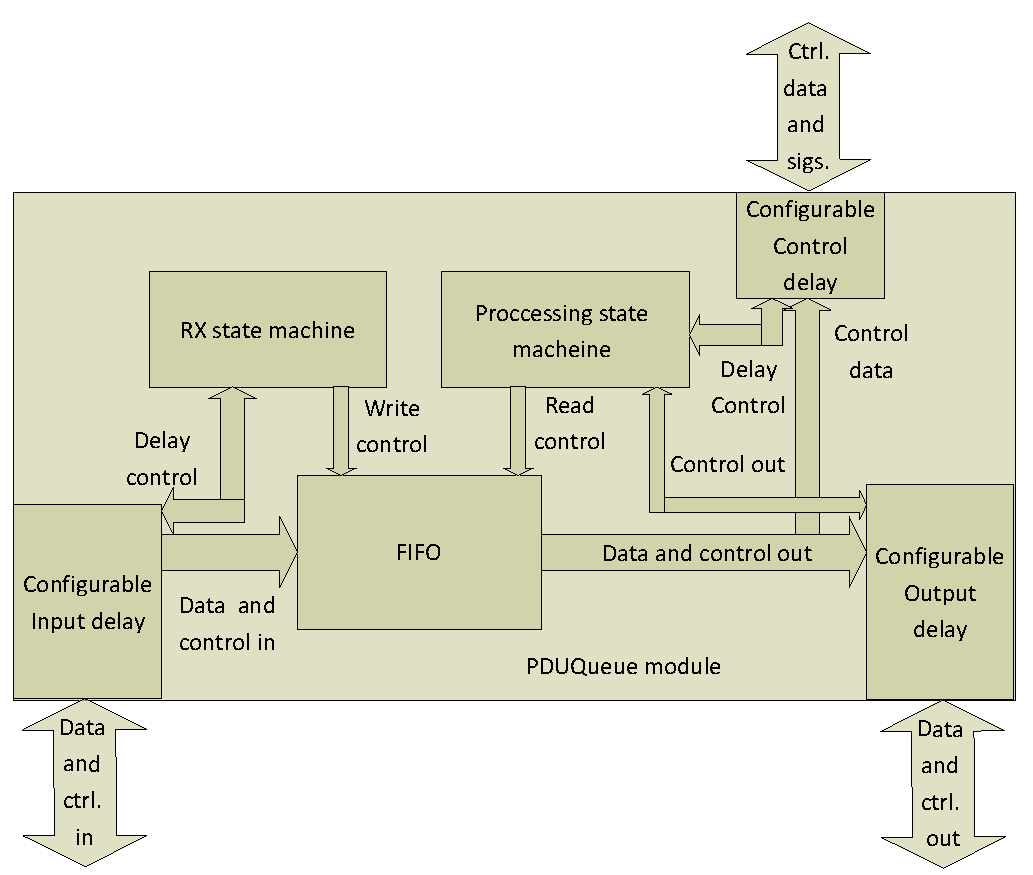
\includegraphics[width=0.5\textwidth]{figures_raw/pdu_queue_imp.pdf}
    \caption{Block diagram of RX part inside of a Protocol Layer module}
    \label{fig:proto_layer_rx_sch}
\end{figure}

The main task of this module is to receive the delimited PDUs and notify the attached controller through the control
interface. The operation cycle is that it forwards the start of the PDU to the controller until it signals its decision
(forward, drop, etc.). The controller is able to pause the operation through the control interface. If the control
decision is `Forward' then the rest of the PDU -- which is essentially the SDU -- is forwarded through the output
interface, while the corresponding control signals are generated as illustrated by Fig.~\ref{fig:data_signals}. In
order to support Out-Of-Band (OOB) signalling, the module has user I/O ports so that the OOB signals are transferred
alongside with the PDU. This overall mechanism provides a generic way to separate the PCI from an SDU, which is a key
part of handling protocol messages.

\subsubsection{Detailed design of `ProtoModule\_TXPart'}

The module depicted on Fig.~\ref{fig:proto_layer_tx_sch} is responsible for accepting data streams of corresponding
PCIs and SDUs and combine them into one single data stream, then forward them through its output interface, which can
be fed into a lower layer `ProtoModule''s SDU input. Since the PDU's PCI and SDU part can be modelled internally as two
separate PDUs, the module described in Section~\ref{subsubsec:PDUQueue_details} can be used for handling the two data
units.
The output of those are fed into another \emph{`PDUQueue'} through a multiplexer. The reassembly control module
virtually operates as a simple internal `protocol' for the 3 \emph{`PDUQueue'}s that always make \emph{`Forward'}
control decision -- hence the note \emph{`PASS\_THROUGH'} on the figure -- and also controls the multiplexer input
selector. Furthermore, the operation supports PCI only transmission cycles as well, which might be desired by some of
the protocols.
%(fig. 20)
\begin{figure}[!htb]
    \centering
    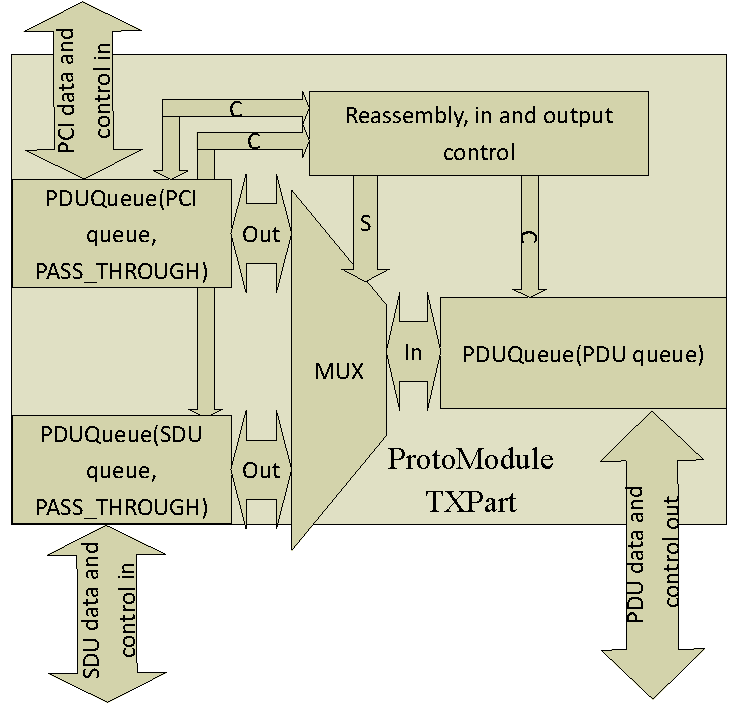
\includegraphics[width=0.35\textwidth]{figures_raw/proto_tx_part_imp.pdf}
    \caption{Block diagram of TX part inside of a Protocol Layer module}
    \label{fig:proto_layer_tx_sch}
\end{figure}

\section{Implementation}\label{sec:Implementation}

The designed framework has been implemented in VHDL with having most of the described parameters as generic inputs of
the components. This design and architecture enables high level of re-usability and customization, which is the main
achievement of this work. Furthermore, since the implementation is open source, it can be modified and/or improved
easily, would there be special requirements that are not covered or unsolvable with the current form of the framework.

For the actual synthesis of the VHDL code on real hardware, a Xilinx Virtex 5 FPGA board -- provided by Aitia
International Inc. -- called SGA-GPlanar \cite{GPlanar} has been used, with a 1 Gbps Ethernet PHY attachment. This
constraint resulted in concrete values for multiple important generic parameters, such as the data bus width or the
clock frequency.
The implementation itself and several test cases are available on \cite{GIT_protolayer}
\url{https://github.com/fecjanky/protolayer} that was used for the verification by simulation and by actual operation
of it.

\begin{figure*}[!htb]
    \centering
    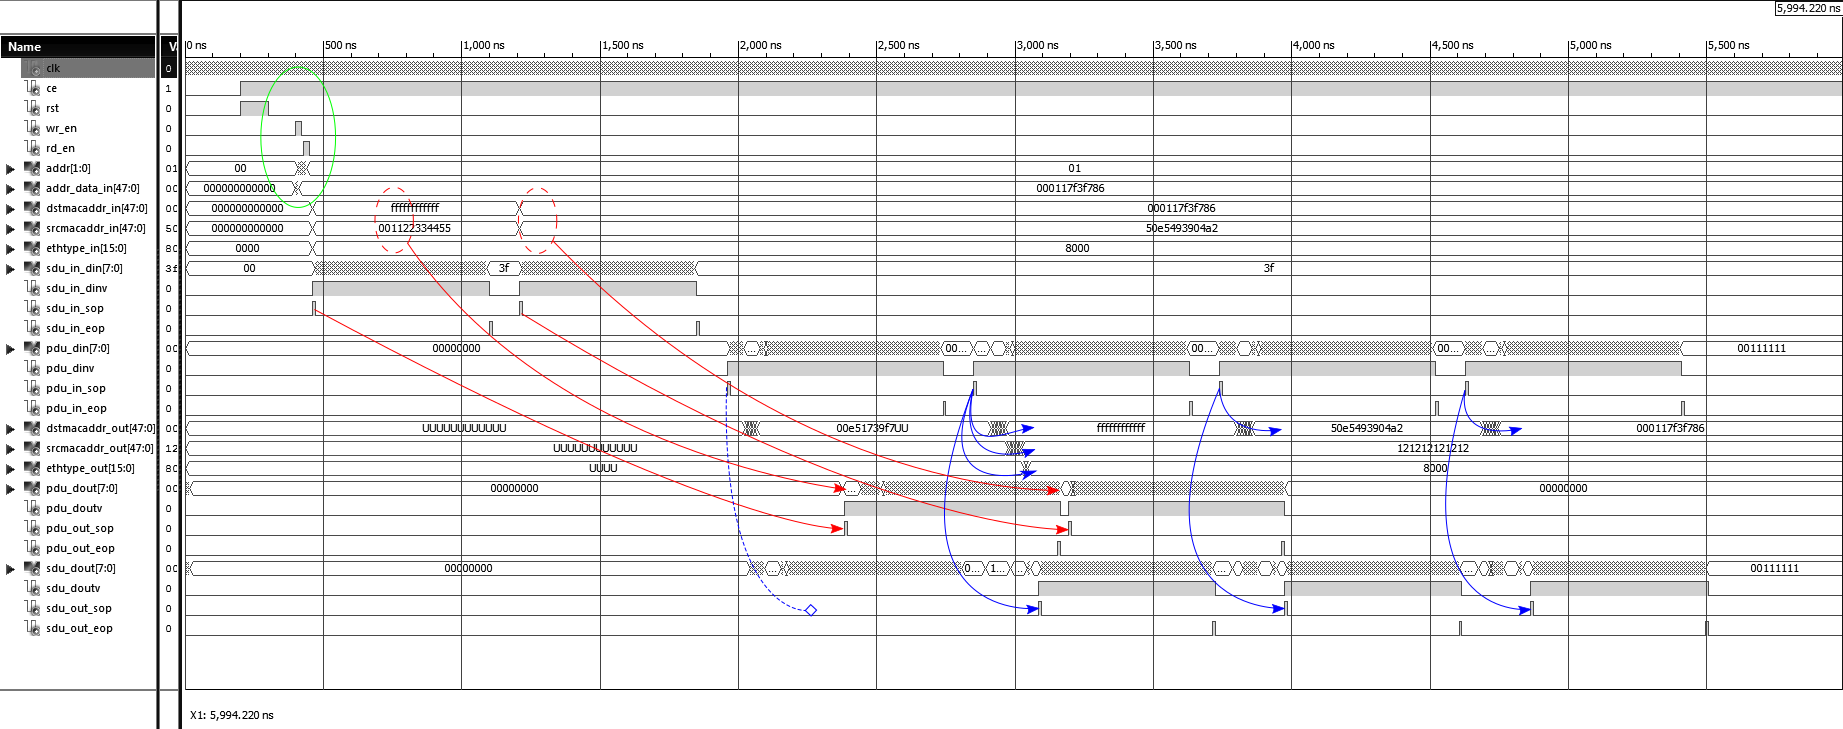
\includegraphics[width=1\textwidth]{figures_raw/ether_tst_wave_annotated.png}
    \caption{Simulation waveform of the Ethernet module exported from Xilinx ISim}
    \label{fig:eth_sim}
\end{figure*}

\section{Verification}\label{sec:Verification}

There were two methods used to verify the design and the implementation:
simulation of the VHDL model using Xilinx ISim, and
synthesis of that on the GPlanar card and interconnecting it with other
devices.

\subsection{Simulation results}

On Fig.~\ref{fig:eth_sim} the simulation waveforms of the Ethernet module can be seen. It illustrates a MAC address
configuration sequence (with read-back) -- green circle -- and sending and receiving multiple PDUs in that order -- the
lines are connecting the corresponding input-output events with \emph{red} colour for transmission and \emph{blue} for
reception of data units. For this specific verification, the module was synthesized with capability to hold 3 station
MAC addresses, of which the station was configured to have two addresses: 50-E5-49-39-04-A2 and a 00-01-17-F3-F7-86.
After completing the configuration sequence, the \emph{MA\_DATA.request} service primitive has been tested with two
data units. These has been followed by testing \emph{MA\_DATA.indication} by feeding four Ethernet II frames to the
lower layer input of the module. Out of the four frames, the :
\begin{itemize}
    \item first was not destined to the station, and
    \item the second was destined to the broadcast address, and
    \item the last to were sent to the configured addresses.
\end{itemize}
It can be seen from the waveforms that the first packet has not been forwarded towards the upper layers -- visible on
the \emph{SDU\_doutv} signal -- and the other were passed up along with all ICI information accompanied by the signals
of Section~\ref{subsec:if_and_func_spec_VHDL}.

\subsection{Packet capture results}

Validation of the ARP (Address Resolution Protocol) module -- that is implemented through the \emph{ProtoLayer} module
-- was performed by interconnecting the device with a Layer 2 switch and operating it on a LAN segment. The module was
able to initiate and respond to address resolution requests. Fig.~\ref{fig:pcap_arp_seq} captures the former case,
where the implementation is performing address resolution of the target host 10.10.0.254. which was a gateway router in
that measurement setting.

\begin{figure}[!htb]
    \centering
    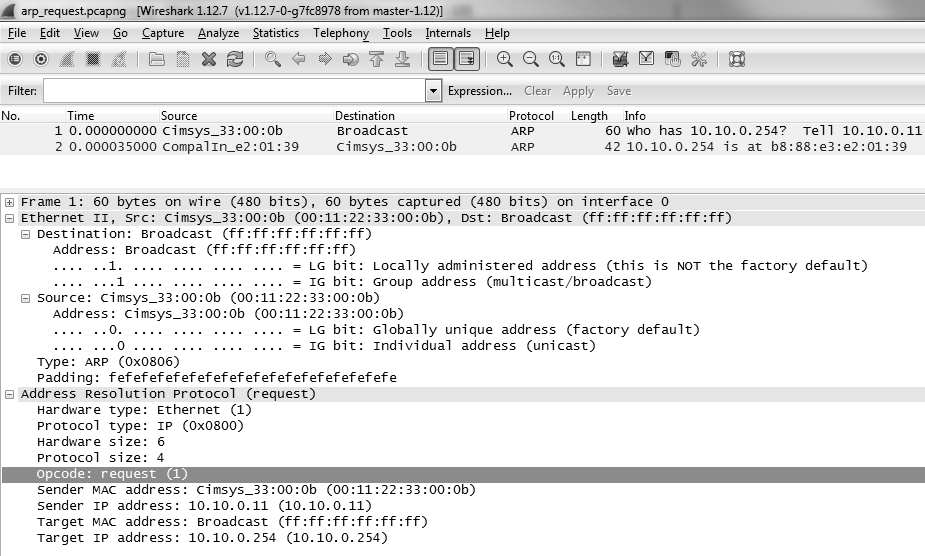
\includegraphics[width=0.5\textwidth]{figures_raw/arp_transaction.png}
    \caption{Packet capture of ARP resolution sequences}
    \label{fig:pcap_arp_seq}
\end{figure}

Based on the numerous and thorough tests -- as well as the two demonstrated simulation and packet capture results --,
it can be stated that the framework design is valid. It can be used to implement various protocols, and it also
satisfies the requirements stated in Section~\ref{sec:Internal Design}.

\section{Conclusion}

The aim of this paper was to present the design and implementation of a generalized framework for FPGA-based networking
systems. This architecture enables high level of re-usability and customization, which is the main achievement of this
work. It is demonstrated that the framework aids implementation of networking protocols using FPGAs and verified that
those can be implemented easily with its support.

The OSI reference model served as a basis for logical and physical structuring of the framework, that by design
addresses layering and interconnection of protocols. The framework has been implemented in VHDL with having nearly all
main parameters as generic inputs that can be tweaked in synthesis time. As part of the verification, the ARP protocol
for
IPv4 and Ethernet has been implemented through the framework as well as the  necessary IEE 802.3 MAC link layer
protocol in full-duplex mode.
At the end of the implementation the framework has been verified by both simulation and synthesizing it on a FPGA based
board equipped with 802.3 PHY interfaces. There were complete,	successful, real world measurements carried out by
interconnecting the board with various devices.

\section*{Acknowledgement}
The author would like to say thanks for AITIA Int’l. Inc. for support, and to Dr. Pal Varga -- the author's mentor --
for his guidance.

% can use a bibliography generated by BibTeX as a .bbl file
% BibTeX documentation can be easily obtained at:
% http://www.ctan.org/tex-archive/biblio/bibtex/contrib/doc/
% The IEEEtran BibTeX style support page is at:
% http://www.michaelshell.org/tex/ieeetran/bibtex/

\bibliographystyle{IEEEtran}
% argument is your BibTeX string definitions and bibliography database(s)
\bibliography{references}

%
% <OR> manually copy in the resultant .bbl file
% set second argument of \begin to the number of references
% (used to reserve space for the reference number labels box)

%\begin{thebibliography}{1}
%
%\bibitem{IEEEhowto:kopka}
%H.~Kopka and P.~W. Daly, \emph{A Guide to \LaTeX}, 3rd~ed.\hskip 1em plus
% 0.5em minus 0.4em\relax Harlow, England: Addison-Wesley, 1999.
%
% \end{thebibliography}

\end{document}
